\section{User Study 1}

% \begin{enumerate}
% \item Process of gameplay
% \item User's feedback for existing games
% \item User's imagination
% \end{enumerate}

In order to realize the current game play experience on google glass. We use games currently existing on google glass to perform our user study. Furthermore, with a view to understanding the response and feedback for different control style and game content from users, we choose four games, ``Balance'', ``Shape Splitter'', ``Matcher'', and ``Clay Shooter'', with unique control type respectively(see Table~\ref{tab:gameControlTypes}).

We recruited 24 users(16 males and 8 females) with average 23.8 years old(std 3.96) and 13.9 years game experience(std 5.96).
To avoid bias caused by myopia, which might affect game expereience if you are not playing google glass with your own shortsight degree lens, we only recruited the user who don't have myopia or wearing contact lens. Moreover, all of our user has no experience wearing google glass before. 

About the process of our user study, we gave user five minutes to play each game, and filled in a questionnaire to understand the positive and negitive feedback from users after playing each game. To make results effective, the order of the game were counterbalanced to eliminate the effects of ordering. After playing all four games, we also provided a final questionnaire to realize the whole glass game play experience from users.

\begin{table}[!h]
\newcommand{\tabincell}[2]{\begin{tabular}{@{}#1@{}}#2\end{tabular}}
   \centering
   \begin{tabular}{|p{0.4\columnwidth}|p{0.4\columnwidth}|}
     \hline
     % \tabhead{Objects} &
     \multicolumn{1}{|p{0.3\columnwidth}|}{\centering\tabhead{Game}} &
     \multicolumn{1}{|p{0.5\columnwidth}|}{\centering\tabhead{Control}} \\
     \hline
     Balance & gyro\\
     \hline
     Shape Splitter & in-air gesture\\
     \hline
     Matcher & gyro, tap\\
     \hline
     Clay Shooter & gyro, voice control\\
     \hline
   \end{tabular}
   \caption{Game control types}
   \label{tab:gameControlTypes}
 \end{table}

\subsection{User feedback}
We collected totally 304 feedback from users(141 positive feedback and 163 negative feedback). After reviewing all feedback, we perceived that some user feedback was not glass related. For instance, user might complain about the level design or visual art, and admired to the innovative game design or music pleasant to hear. Thus, we organized all user feedback into 16 categories(see Table \ref{tab:issueType}). We removed user feedback which were unrelated to glass. After that, we remained 131 feedback with 45 positive feedback and 86 negative feedback. 
We summerized all feedback issues in Table \ref{tab:result1} and briefly divided all negative feedback into 6 main issue categories, which are ``Gyro'', ``In-Air Gesture'', ``Voice control'', ``Eye Tiring'', ``Social Acceptable'', and ``Tapping''(see Figure~\ref{fig:negativeFeedback}).


\subsection{New issue with glass}
According to the negative feedback from user(see Figure~\ref{fig:negativeFeedback}), issues of gyro, in-air gesture, voice control and tapping are all part of control issue. We integrated them into ``Limited control'' category. So we can conclude three new issues, ``Limited control'', ``Eye tiring'' and ``Social acceptable'' which are not exist in traditional game design for google glass game design.

\begin{enumerate}
\item Limited control: On google glass compared to other games, there is no effective powerful input such as mouse, keyboard, joystick or touch screen. However, There are some non-traditional gaming input such as camera, small touch pad, microphone, gyroscope, and accelerometer. How to use these new control in glass game design is still an open question for people to discuss and explore.
% affective powerful gaming input?

\item Eye tiring: Different from traditional gaming platform, playing game on glass need more intence of eye muscle. User reported that it is really easy and quick to feel eye tiring. With this consideration, game design on google glass should control the gaming duration really carefully. It is not practical to let users focus on glass for a long time.

\item Social acceptable: Although we can use voice control and in-air gesture on google glass, user may have different feeling in different environment, affected by people around the user. So we have to use these control issues carefully, and check out whether our control scheme is social acceptable.

\end{enumerate}


%And we can briefly divide the negative feedback into 6 main issue categories``Limited control'', ``Eye tiring'' and ``Social acceptable''(see Figure~\ref{fig:negativeFeedback}), which are not exist in traditional game design.

\begin{table}[!h]
\newcommand{\tabincell}[2]{\begin{tabular}{@{}#1@{}}#2\end{tabular}}
   \centering
   \begin{tabular}{|p{0.4\columnwidth}|p{0.4\columnwidth}|}
     \hline
     % \tabhead{Objects} &
     \multicolumn{1}{|p{0.3\columnwidth}|}{Issue} &
     \multicolumn{1}{|p{0.5\columnwidth}|}{User Feedback} \\
     % \multicolumn{1}{|p{0.3\columnwidth}|}{\centering\tabhead{Game Play Feedback}} &
     % \multicolumn{1}{|p{0.5\columnwidth}|}{\centering\tabhead{User Feedback}} \\
     \hline
     \multicolumn{1}{|p{0.3\columnwidth}|}{Eye Tiring} & 
     \multicolumn{1}{|p{0.5\columnwidth}|}{p1: Eyes need to focus on the screen all the time, which require to exert high strength on eye muscle. p2: Muscle below eyelids will feel uncomfortable for long time gazing at the glass screen.} \\
     % p1:一直聚焦在畫面上眼睛很酸,眼睛需要很用力聚焦在上面。\\p2: 眼睛很酸,需要一直注視畫面很不舒服,眼皮下方肌肉會酸。} \\
     \hline
     \multicolumn{1}{|p{0.3\columnwidth}|}{Gyro is comfortable for 1D and 2D control } & 
     \multicolumn{1}{|p{0.5\columnwidth}|}{p3: Sensing by gyro is intuitive for users. If user tilts his head to one side, he will know what need to do. p4: Using head to aim, and this manipulation method is intuition.} \\
     % p3:Gyro感應蠻直覺的,知道頭往哪邊歪,他應該會怎麼做 \\p4:用頭去瞄準,這操作很直覺。
     \hline
     \multicolumn{1}{|p{0.3\columnwidth}|}{Gyro with 360 degree is BAD} & 
     \multicolumn{1}{|p{0.5\columnwidth}|}{p5: Head needs to turn around back and forth, and the turing extent needs enormous. p6: User has no idea why needs to turn a round.} \\
     % p5:頭要轉來轉去,轉的幅度要很大 \\p6:繞一圈不知道要幹嘛。
     \hline
     \multicolumn{1}{|p{0.3\columnwidth}|}{Voice Control \& In-Air Gesture are NOT social acceptable} & 
     \multicolumn{1}{|p{0.5\columnwidth}|}{p7: Users will fell shy while using voice control to play, and it will catch passerby's attention. p8: If user slices fruit in front of google glass screen, no one knows what does the user do. In other words, it's a little bit foolish while doing this movement.} \\
     % p7:用聲控有點害羞。在路邊應該會引人側目。\\ p8:別人看不到我在切什麼。手舉在空中亂畫很蠢。
     \hline
     \multicolumn{1}{|p{0.3\columnwidth}|}{Tappings as main control are annoying} & 
     \multicolumn{1}{|p{0.5\columnwidth}|}{p9: User needs to put their hand by the side of user's head. It will make user's hand uncomfortable for a long time and screen will shake while taking a photo by tapping. p10: It's really tired for user to maintain hand posture all the time.} \\
     % p9:手要一直放在頭旁邊,很酸,而且拍的時候畫面會震動。 \\p10:手一直維持這個肢勢很累
     \hline
     \multicolumn{1}{|p{0.3\columnwidth}|}{In air gesture is tiring} & 
     \multicolumn{1}{|p{0.5\columnwidth}|}{p11: It will feel uncomfortable for user raising his hands in front of his eyes all the time. p12: After playing a period of time, user's hand will feel really sore and do not want to raise his hands anymore.} \\
     % p11:手要一直舉在眼前,手會很酸。 \\p12:玩到後面手很酸,會不想把手抬起來。
     \hline
     \multicolumn{1}{|p{0.3\columnwidth}|}{Current in air gesture detecting is imprecise} & 
     \multicolumn{1}{|p{0.5\columnwidth}|}{p13: The relationship between hands waving and screen response is really loose. In other words, the position where user's hands wave is separate with the position where the knife slices. p14: User can't know the scope of the camera, which make the scope of manipulation is really blurred.} \\
     % p13:手揮的動作跟畫面上的反應,關係非常的loose。你揮的位置跟砍的位置完全分開。\\p14:我無法掌握攝影機的範圍,操作範圍非常模糊。
     \hline
     \multicolumn{1}{|p{0.3\columnwidth}|}{Voice control always out of control} & 
     \multicolumn{1}{|p{0.5\columnwidth}|}{p15: Google glass can't identidy the source of the sound, which is from the user or the environment. p16: Google glass is easy to be interrupted from the environment. For instance, any sound will let ball to throw out.} \\
     % p15:他不能去分出是旁邊的噪音還是我發出的。 \\p16:會輕鬆的被干擾,發出任何聲音球都會跑出去。
     \hline
   \end{tabular}
   \caption{We collect 304 feedbacks and manually divide into 16 categories.}
   \label{tab:issueType}
 \end{table}


% \begin{table}[!h]
% \newcommand{\tabincell}[2]{\begin{tabular}{@{}#1@{}}#2\end{tabular}}
%    \centering
%    \begin{tabular}{|p{0.4\columnwidth}|p{0.3\columnwidth}|}
%      \hline
%      % \tabhead{Objects} &
%      \multicolumn{1}{|p{0.3\columnwidth}|}{\centering\tabhead{Issue}} &
%      \multicolumn{1}{|p{0.5\columnwidth}|}{\centering\tabhead{User Feedback}} \\
%      \hline
%      Eye Tiring & \tabincell{c}{
%      p1: Eyes need to focus on the screen all the time, which require to exert high strength on eye muscle.\\p2: Muscle below eyelids will feel uncomfortable for long time gazing at the glass screen.} \\
%      % p1:一直聚焦在畫面上眼睛很酸,眼睛需要很用力聚焦在上面。\\p2: 眼睛很酸,需要一直注視畫面很不舒服,眼皮下方肌肉會酸。} \\
%      \hline
%      Gyro is comfortable for 1D and 2D control & \\p3:Gyro感應蠻直覺的,知道頭往哪邊歪,他應該會怎麼做 \\p4:用頭去瞄準,這操作很直覺。
%      \hline
%      Gyro with 360 degree is BAD & \\p5:頭要轉來轉去,轉的幅度要很大 \\p6:繞一圈不知道要幹嘛。
%      \hline
%      Voice Control \& In-Air Gesture are NOT social acceptable & \\ p7:用聲控有點害羞。在路邊應該會引人側目。\\ p8:別人看不到我在切什麼。手舉在空中亂畫很蠢。
%      \hline
%      Tappings as main control are annoying & \\ p9:手要一直放在頭旁邊,很酸,而且拍的時候畫面會震動。 \\p10:手一直維持這個肢勢很累
%      \hline
%      In air gesture is tiring & \\ p11:手要一直舉在眼前,手會很酸。 \\p12:玩到後面手很酸,會不想把手抬起來。
%      \hline
%      Current in air gesture detecting is imprecise & \\ p13:手揮的動作跟畫面上的反應,關係非常的loose。你揮的位置跟砍的位置完全分開。\\p14:我無法掌握攝影機的範圍,操作範圍非常模糊。
%      \hline
%      Voice control always out of control & \\ p15:他不能去分出是旁邊的噪音還是我發出的。 
%      \\p16:會輕鬆的被干擾,發出任何聲音球都會跑出去。
%      \hline
%    \end{tabular}
%    \caption{Small Sun.}
%    \label{tab:result1}
%  \end{table}

 \begin{table}[!h]
\newcommand{\tabincell}[2]{\begin{tabular}{@{}#1@{}}#2\end{tabular}}
   \centering
   \begin{tabular}{|p{0.4\columnwidth}|p{0.3\columnwidth}|}
     \hline
     % \tabhead{Objects} &
     \multicolumn{1}{|p{0.3\columnwidth}|}{Traditional issue} &
     \multicolumn{1}{|p{0.5\columnwidth}|}{Level design, Music, Visual art, Casual, Challenge, Game for purpose, Innovative, Physics, Immersion} \\
     % \multicolumn{1}{|p{0.3\columnwidth}|}{\centering\tabhead{Game Play Feedback}} &
     % \multicolumn{1}{|p{0.5\columnwidth}|}{\centering\tabhead{User Feedback}} \\
     \hline
     \multicolumn{1}{|p{0.3\columnwidth}|}{Glass related issue} & 
     \multicolumn{1}{|p{0.5\columnwidth}|}{Gyro, In-air gesture, Tap, Voice control, Eye tiring, Social acceptable, AR} \\
     \hline
   \end{tabular}
   \caption{We collect 304 feedbacks and manually divide into 16 categories.}
   \label{tab:issueType}
 \end{table}

% \begin{table}
% \newcommand{\tabincell}[2]{\begin{tabular}{@{}#1@{}}#2\end{tabular}}
%   \centering
%   \begin{tabular}{|c|c|c|}\hline
% 1 & \tabincell{c}{the first line \\ the next\\the next\\ last} & \tabincell{c}{one \\ one}\\\hline
% 2 & \tabincell{c}{hello\\ aha\\ ok \\yes \\en} & \tabincell{c}{two \\ two \\ two} \\\hline
% \end{tabular}
%   \caption{longtitle}
% \end{table}

\begin{figure}[!t]
\centering
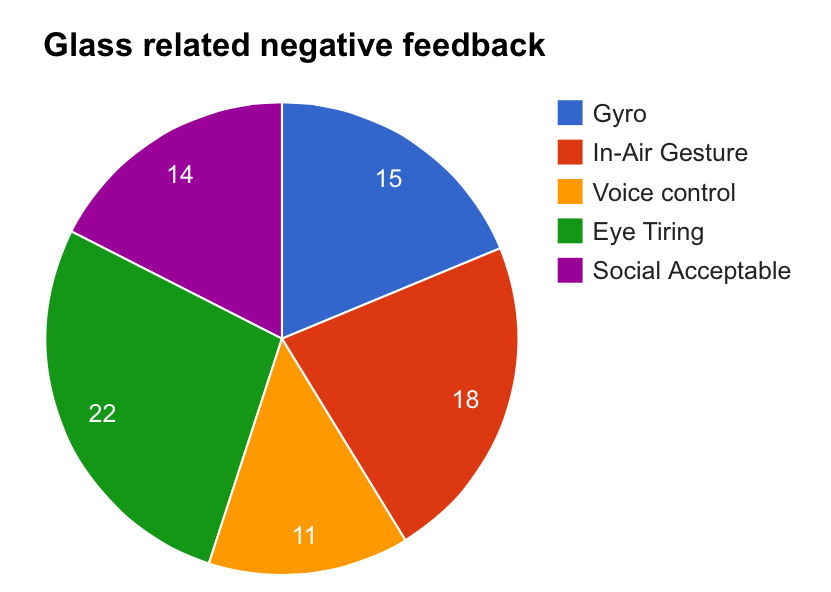
\includegraphics[width=0.9\columnwidth]{Figures/US1_userfeedbackStatistics.png}
\caption{We catogorize glass related negative feedback into 6 categories. Gyro, In-Air Gesture, Voice control and Tapping are all part of control issue.}
\label{fig:negativeFeedback}
\end{figure}


%\subsection{Observation}
% \begin{enumerate}
% \item NOT social acceptable != NOT fun
% \item Small movement is better
% \end{enumerate}
%From user feedback, although social acceptable would make an influence on glass game play experience, most users still think game play experience is fun and interesting. With this condition, we can conclude that social acceptable is independent to the level of fun and enjoyment. In other words, if a game has low social acceptable rate, it does not mean the game is not fun or users don't like it. In addition, we also find that small movement interacting with google glass is better and more perferred for users. 


\subsection{User imagination}
After playing all four games,in our final interview we also asked users to imagine what kind of games on google glass will they like the most and why. With the previous gaming experience in user study 1, they brought up thirty-seven insteresting glass game idea in total. We divided them into six types of game, ``First-Person Shooter'', ``Reality Puzzle Game'', ``Social Game'', ``Sport Game'', ``Management Game'', and ``Others'' respectively (see Figure~\ref{fig:US1_TypesOfGame}). We found that one-third of users want like first-person shooter game the most. We list the reason why users think these type of game is suitable for google glass.

 

\begin{enumerate}
\item FPS : They think google glass is a native first-person view, will be really suitable for First-Person Shooter. And some of user imagine that they can use mobile phone, which is always connected with glass, as an input device(with gun metaphor) to extend the limited input power.

\item Reality Puzzle Game : Some user suggest not focusing on glass screen, we can focus on the real world. Like playing reality puzzle game, player can get hint from google glass, but player doesn't need to focus on glass screen all the time. 

\item Sport Game : Users think google glass can be a gamification tool for sport. It's a see-through screen, we can check google glass even though on exercising. Google Glass can analyze GPS or accelerometer information to give the player reward message to make exercising more fun and enjoyment.

\item Social Game : To be continued.....

\item Management Game : With the characteristic of Always-On, Users think google glass is really suitable for management game(or Pet-Nurturing Game).Player can check the game status any time with a glance, and doing some simple command with tapping. And these type of game is short gaming period, doesn't need heavy control.

\end{enumerate}


%After playing all four games,in our final interview we also asked users to imagine what kind of games on google glass will they like the most in user study 1. With existing glass game scene and users' originality, they brought up thirty-seven interesting glass game scenario in total. We divided them into six types of game, ``First-Person Shooter'', ``Reality Puzzle Game'', ``Social Game'', ``Sport Game'', ``Management Game'', and ``Others'' respectively (see Figure~\ref{fig:US1_TypesOfGame}). We also found that one-third of users want like first-person shooter game the most. So we decided to implement a first-person shooter game which will support multiple types of control style for users. With this design, not only users can choose which control type they like the most by their own, but we also can find out the best control style from users' feedback for first-person game on google glass and design a guideline to make better game play experience.

\begin{figure}[!t]
\centering
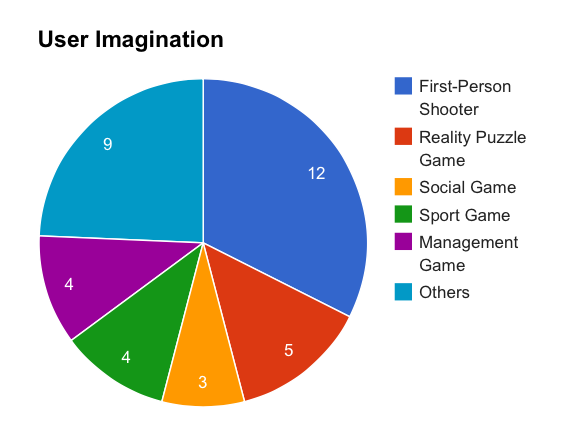
\includegraphics[width=0.9\columnwidth]{Figures/US1_userImaginationStatistics.png}
\caption{Hi I'm Small Sun 2.}
\label{fig:US1_TypesOfGame}
\end{figure}
